%\iffalse
% \begin{frame}{Why solve these problems?}
% \begin{itemize}
%   \item <+-> {\color{red}Matrix-vector multiplication} on geometric
%     graphs appears in the $n$-body simulation problem, a notable
%     problem in physics. For example, let's say you want to calculate the
%     gravitational force of a system of planets on each planet. How can
%     you compute this quickly?
%   \begin{itemize}
%     \item <+-> This can be solved with a matrix-vector product using the
%       $K$-graph, where $K(x,y) = \frac{1}{\|x-y\|_2^2}$ (exercise for
%       listener). 
%     \item <+-> The fast multipole method solves this problem quickly for certain $K$ in
%       low dimension. Can we extend this method to different $K$ and
%       different dimension? Can we improve the fast multipole method's run time?
%   \end{itemize}
%   \item <+->Fast {\color{darkblue} spectral sparsifiers}
%     mean to fast algorithms, for problems
%     including: spectral clustering, max-flow, sparsest cut, min-cut. For
%     any graph you can sparsify in almost-linear time, you can
%     approximate the above problems in almost-linear time.
%   \item <+-> {\color{darkgreen}Laplacian solvers} on geometric graphs have applications to
%     semi-supervised learning, a common task in machine learning.
% \end{itemize}
% \end{frame}

\begin{frame}{Why solve these problems?}

  {\color{red}Matrix-vector multiplication}, {\color{darkblue}Spectral
  Sparsifiers}, {\color{darkgreen} Laplacian Solvers}
\begin{itemize}
  \item <+-> The problems we tackle are fundamental linear algebra
    questions.
  \item <+-> Geometric graphs are common in computer science. They
    appear in fields
    ranging from: 
    \begin{itemize}
      \item Computational geometry
      \item Machine learning
      \item Image recognition
      \item physics simulations, and more.
    \end{itemize}
  \item <+-> It seems natural to find fast algorithms and hardness
    results for fundamental linear algebra problems on these graphs.
\end{itemize}
\end{frame}

\begin{frame}{Why solve these problems?}

  {\color{red}Matrix-vector multiplication}, {\color{darkblue}Spectral
  Sparsifiers}, {\color{darkgreen} Laplacian Solvers}
  \begin{itemize} 
    \item We have hardness results on {\color{red}matrix vector
      multiplication.} In particular, it is hard to approximate the
      matrix-vector multiplication on most $K$-graphs in faster than
      $O(n^2)$  time.
    \item Our hardness work for {\color{red}matrix vector multiplication} proves that the \textbf{fast
  multipole method} must have exponential dependence on $d$. 
  \item This is a famous method in computer science, used in physics
    simulations to find gravitational forces on a planet given $n$
      planets in $d$ dimensional space.
  \end{itemize}
\end{frame}

  \begin{frame}
    \frametitle{Interlude: Fast Multipole Method}
  \only{
  \begin{center}
  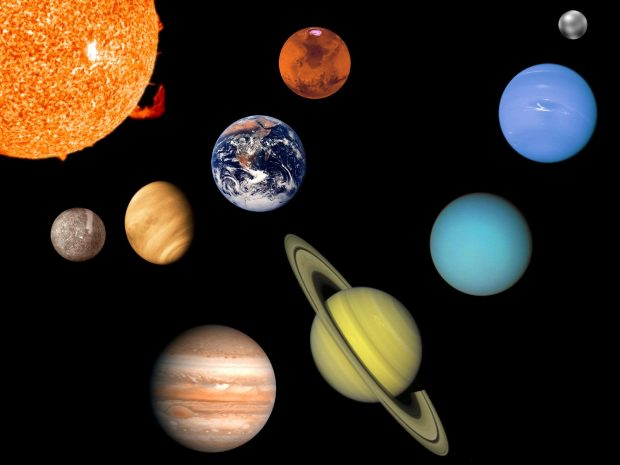
\includegraphics[width=.7\textwidth]{figs/solar-system-0.jpg}
  \end{center}
  }
\end{frame}
\begin{frame}
    \frametitle{Interlude: Fast Multipole Method}
  \only{
  \begin{center}
  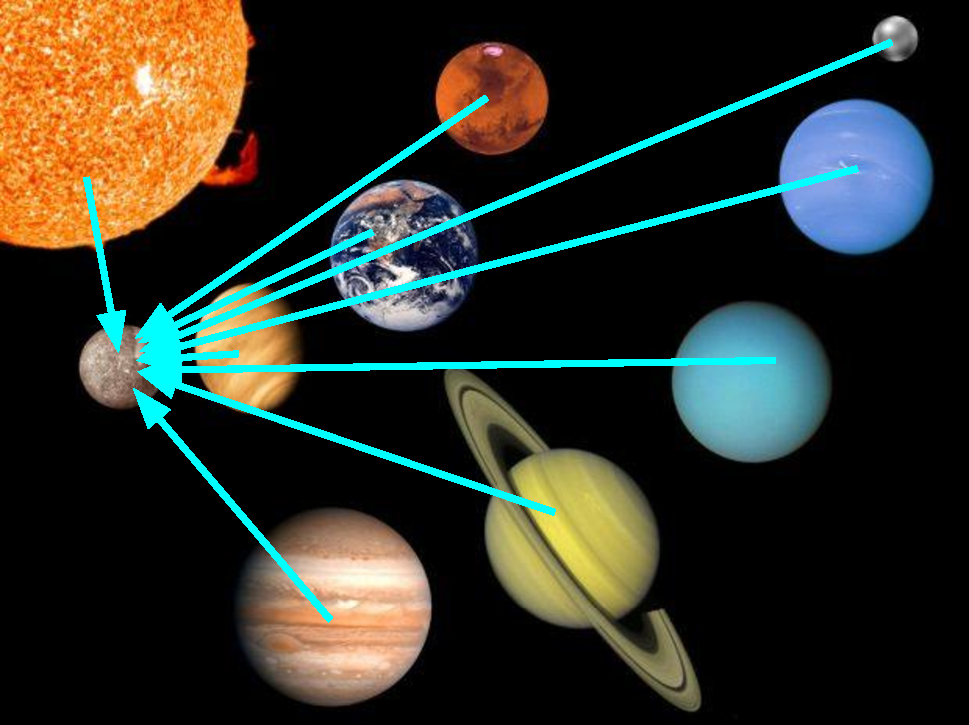
\includegraphics[width=.7\textwidth]{figs/solar-system-1.pdf}
  }
  \end{center}
  \begin{itemize}
    \item Computing the gravitational force on one planet is $O(n)$.
  \end{itemize}
\end{frame}
\begin{frame}
    \frametitle{Interlude: Fast Multipole Method}
    \begin{itemize} 
      \item How about all planets?
      \item Naively, it will take $O(n^2)$ time to compute the
        gravitational force on all planets.
      \item The Fast multipole method (GR 85) shows how to approximate
        this in $O(n2^{O(d)}$ time.
      \item When $d$ is small, this is good. Is it possible to do
        better?
      \item Our hardness work on {\color{red} Matrix Vector
        Multiplication} shows the answer is no!
    \end{itemize}
\end{frame}
\begin{frame}
    \frametitle{Interlude: Fast Multipole Method}
    \begin{itemize} 
      \item What does fast multipole method do with matrix vector
        multiplication?
      \item \begin{center}
    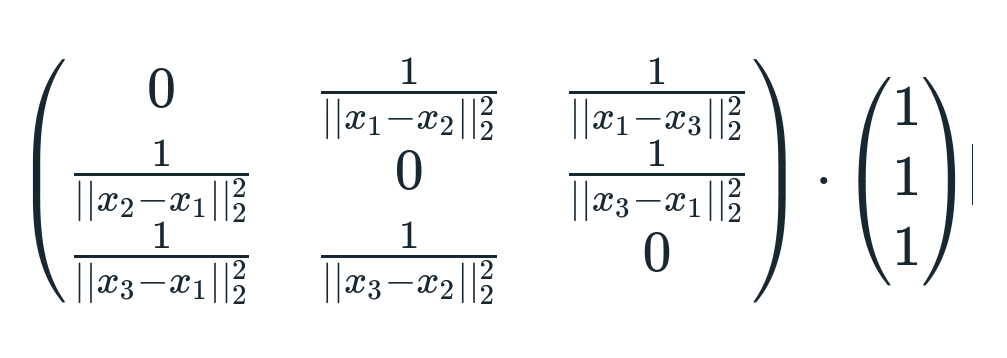
\includegraphics[width=1\textwidth]{figs/mv2.png}
        \end{center}

    \end{itemize}
\end{frame}

\begin{frame}
  \frametitle{Why solve these problems?}

  {\color{red}Matrix-vector multiplication}, \textbf{{\color{darkblue}Spectral
  Sparsifiers}}, {\color{darkgreen} Laplacian Solvers}
  \begin{itemize} 
    \item Why is computing fast spectral sparsifiers important?
    \item Fast sparsifiers (roughly $O(nd)$ time to compute) imply
      roughly $O(nd)$ time algorihtms for:
      \begin{itemize}
        \item Maximum Flow.
        \item Minimum Cut.
        \item Sparsest Cut. Given a graph, how can you cut a small
          number of edges to split it into roughly balanced components?
        \item Balanced Cut.
        \item Effective resistance computations. 
      \end{itemize}
    \item You can even do some fast machine learning (spectral
      clustering) with spectral sparsifiers!
  \end{itemize}
\end{frame}
